\documentclass{report}
% Packages
\usepackage{titlesec}
\usepackage{graphicx}
\usepackage{lipsum} % For dummy text, you can remove this
\usepackage[style=numeric, backend=biber]{biblatex} % Import the package for reading .bib files
\addbibresource{Communication.bib} % Add the .bib file

% Title page
\title{Dissertation Title}
\author{Luis Yallico Ylquimiche}
\date{\today}

\begin{document}

% Title page
\maketitle

% Abstract
\begin{abstract}
LOREM IPSUM
\end{abstract}

% Table of contents
\tableofcontents

% Chapters
\chapter{Introduction}
\section{Background}
\lipsum[1-2] % Replace with your content

\chapter{Literature Review}
\section{Previous Studies}
\lipsum[3-4] % Replace with your content

\chapter{Implementation}

\section{ESP-IDF}
Why use ESP-IDF over Arduino IDE in this project? \cite{esp-boards_esp-idf_nodate}\cite{expressif_freertos_nodate}

As we are using a ESP32 microcontroller to build our swarm, which left us with two options to program it: Arduino IDE or ESP-IDF. The reasons we chose the latter are because, first, it is the official development framework for the ESP32 microcontrollers, this means that ESP-IDF is native to ESP32 whereas Arduino is an API wrap around ESP-IDF. Making ESP-IDF more stable and enabling more advanced features, specially for communication data links such as Bluetooth, Wifi and LORA. Secondly, it is more powerful and flexible than Arduino IDE, because it allows the use of FreeRTOS which allows multi core development support (our M5 Stack has two cores) and is a pre-requisite for running microROS in the ESP32 microcontroller (at the time of writing this microROS does not support Arduino), hence making it more suitable for complex projects like this one. Thirdly, it is more efficient in terms of memory and speed (as it enables parallel processing) which is important for a project that requires real-time communication between multiple devices in a swarm. Finally, it is more professional and an industry standard, it allows dependency tracking, Over the Air (OTA) updates, unit testing, enhanced debugging and comprehensive documentation around it, which means it is more likely to be supported in the future and software is less likely to become deprecated over time.

How was the WIFI implementation done?

We utilized the built-in WiFi capabilities of the ESP32 with the ESPNOW communication protocol, which supports multiple unicast connections. While ESPNOW can theoretically handle around 20 devices simultaneously, practical limits are dictated by environmental factors. Additionally, ESPNOW enables multicast data transmission to multiple devices on the same channel, which can be used to pair devices or send messages to multiple swarm members. The protocol operates at a default bitrate of approximately 1 Mbps, although a portion of this bandwidth is consumed by necessary overhead, such as the MAC header. For our implementation, each swarm robot was pre-configured with the MAC addresses of all peers to facilitate direct communication. %might need to add multicast implementation
One key aspect to point out in this implementation is that connection handling and device pairing, which oversees how swarm members join and leave a connection. In its most basic form, we created a loop that goes over each MAC address and tries to rely a direct message to each other member in the swarm, to server as our benchmark. It is understood that the implications of this can have an impact on data loss and latency of the network.
For expanding a swarm dynamically, cryptographic keys might be needed to securely onboard new members, this however is out of scope of the current study.

How was the IR implementation achieved?

Using the IR board, described previously. We connected the M5Stack via the external I2C port, furthermore we had to use the Arduino library as a component of the ESP-IDF implementation for the this to work, this was due to compatibility issues between ESP-IDF and Arduino libraries. The board itself is running with an Arduino Nano to process the IR signals into messages and then sending this data accross via the SDA/SCL pins. One major implication for this, was the need to change the FreeRTOS clock speed from 100Hz to 1000Hz which improves responsiveness but at the cost of higher CPU load and power consumption. Some key parameters also include the frequency if the I2C itself which was set at 100kHtz and the master/slave configuration (M5 being the master device), this is initialized from the M5 once powered on after the 5V bus is switched on (to power the board). For more details regarding the IR board implementation please see X. 

\section{OTA}


%TODO: include references
Integrating Over-the-Air (OTA) updates into robotic swarms improves efficiency in deploying and managing software, especially in remote or hazardous environments like space or disaster zones. This scalable approach allows remote management of the entire fleet, ensuring all robots consistently run the latest software. For instance, in the automotive sector Tesla's software-enabled feature activation model showcases how OTA updates can enhance customer services and streamline hardware production by allowing quick, widespread deployment of critical updates.

Using cloud services like AWS S3 for hosting OTA updates ensures high availability and safe rollback capabilities in our system, increasing robustness against failures like incomplete updates due to power loss. This setup reduces capital expenditure costs and improves swarm scalability compared to local servers that can become a single source of failure. Mirroring Apple’s use of cloud infrastructure for massive, global iOS updates—but also complies with regional data laws by using decentralized storage and managed encryption.

Our project integrates Continuous Integration and Deployment (CI/CD) to maintain dynamic software development for the swarm. This ensures that features and fixes are promptly integrated and tested, maintaining software quality and allowing the swarm to consistently operate with the latest releases. This approach is crucial for testing various communication parameters within our experiments, ensuring reliable and systematic updates.

\begin{figure}[h]
    \centering
    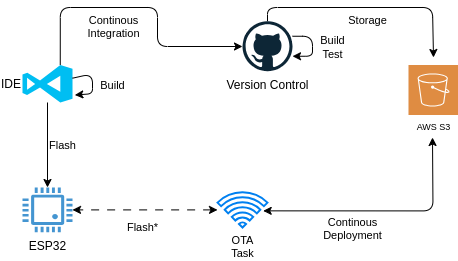
\includegraphics[width=0.5\textwidth]{architecture.png}
    \caption{System Architecture}
    \label{fig:architecture}
\end{figure}

Figure \ref{fig:architecture} shows the implementation of our system to enable over the air updates (OTA) and continuous integration \& continuous deployment (CI/CD) framework over the swarm. 
\begin{itemize}
    \item \textbf{Local Development Environment}: ESP32 application development takes place locally using VSCode, the IDE environment uses version 5.2.2 of ESP-IDF and Python 3.11 to build and flash the code in-situ to the ESP32 module. This self contained development environment allows for testing new features and updates without affecting previous versions of the application running on the swarm.
    \item \textbf{Version Control System \& CI/CD}: The codebase is stored in a public repository on GitHub: \url{https://github.com/yallico/robotics_dissertation}, this allows for version control and automates the build and test process upon every commit. The ESP32 project is compiled and it generates the .bin binary file used for OTA. This process ensures that the codebase is always in a working state and ready for deployment.
    \item \textbf{Cloud Storage}: Once the OTA binary file is generated, it is uploaded to an AWS S3 public bucket. S3 serves as a reliable and low cost storage solution for the OTA updates. We decided to leave encryption and access control out of scope from the OTA implementation, yet we acknowledge that encryption is a non-trivial task that swarms should consider when deploying OTA updates in terms of computational resources required and security implications in industry. %TODO: Add reference to encryption in OTA
    \item \textbf{OTA Update Process}: The ESP32, runs a task that is triggered upon initialisation which compares its current application version against the latest version available in S3. If the version in AWS S3 diverges from the current version running in the ESP32. It then downloads the .bin file and performs the update following OTA best practice (see Section X). %TODO: Add reference to OTA best guidance from ESP-IDF.

\end{itemize}


\section{Experimental Setup}
\lipsum[5-6] % Replace with your content

% Add more chapters as needed

\newpage
\printbibliography

\end{document}